\documentclass{article}

\usepackage[dblblindworkshop]{neurips_2026}
\workshoptitle{XAI4Science: Knowledge Discovery and Trust through Interpretable Foundation Models}

\usepackage[utf8]{inputenc}
\usepackage[T1]{fontenc}
\usepackage{hyperref}
\usepackage{url}
\usepackage{booktabs}
\usepackage{amsfonts}
\usepackage{amsmath}
\usepackage{nicefrac}
\usepackage{microtype}
\usepackage{xcolor}
\usepackage{graphicx}

\title{Causal Steering of Protein Language Models: \\
When Correlational Validation Fails, and How to Catch It}

\author{%
  Anonymous Author(s) \\
  Anonymous Institution \\
  \texttt{anonymous@anonymous.edu}
}

\begin{document}

\maketitle

\begin{abstract}
Foundation models for biology are increasingly probed with interpretability
methods that identify correlational structure -- an attention head that
aligns with a known biological signal, a scoring proxy that correlates
with real experimental labels -- and this correlational structure is
often treated as evidence that a targeted causal intervention (activation
steering, attribution-guided editing) will work as intended. We test this
assumption directly on a protein language model, ESM2-650M, using
difference-of-means activation steering, a causal intervention already
shown to work for one property (thermostability). Under a pre-registered
six-criterion protocol testing five novel target properties, we find no
positive relationship between proxy validity and causal steering effect:
our best-validated proxy (binding affinity, $r=0.80$ held-out, confirmed
by a weight-shuffle null control) steers nothing, while a substantially
weaker proxy ($r=0.22$, catalytic activity) produces a robust,
three-seed-replicated causal effect. An independent, component-level
mechanistic-interpretability result shows the identical pattern one level
down: attention heads ranked by correlation with real 3D protein contacts
show near-zero relationship to their causal ablation effect, confirmed
via a full 480-head sweep. We further show that a single evaluation seed
can produce a misleading verdict on a specific robustness criterion even
when the underlying causal effect is stable, and introduce a diagnostic
-- steering-vector cosine similarity across targets -- that explains an
otherwise-unexplained result as a geometric artifact of a different,
validated causal direction rather than independent evidence. These
findings argue for validating explanation methods against downstream
causal interventions, not treating correlational salience as
self-certifying.
\end{abstract}

\section{Introduction}

A foundation model's internal correlational structure -- which attention
heads track a known signal, which features predict a real label -- is
frequently used as the basis for a claimed causal intervention: ablate
this head because it looks important, steer along this direction because
it correlates with the target property. Whether that correlational
salience actually predicts the intervention's causal effect is rarely
tested directly. We test it on ESM2-650M, a protein language model, using
difference-of-means activation steering \citep{huang2025steering}, a
method already validated to causally move a real biological property
(thermostability) by adding a direction -- built from the residual-stream
activation difference between real high- and low-property sequence
groups -- to the model during generation.

We ask: does a scoring proxy's correlation with real experimental labels
predict whether steering toward it causally works? Across five novel
target properties under one pre-registered protocol, the answer is no,
and not weakly so. The best-validated proxy in our study ($r=0.80$
held-out, for binding affinity) produces a flat null causal effect at
every tested intervention strength, while a substantially weaker proxy
($r=0.22$, catalytic activity) produces a clean, monotonic effect that
replicates across three independent random seeds. This mirrors an
independent, purely mechanistic-interpretability result in the same
model family: \citet{vig2021bertology} identified an attention head whose
attention pattern correlates 12.9$\times$ with real 3D residue contacts,
explicitly noting this was never tested causally; we ablate it directly
and find an effect statistically indistinguishable from a low-correlation
control, confirmed by a full sweep of all 480 heads in the model. Two
levels -- individual components and entire target properties -- one
lesson: correlational salience, however striking, is evidence about a
model's learned representations, not a certificate that an intervention
built on it will causally succeed.

\section{Method: A Pre-Registered Protocol for Causal Validation}
\label{sec:method}

Before testing any target property, we lock a six-criterion decision
rule, applied uniformly and computed automatically: (1) the real steering
direction significantly beats a matched-norm random-direction control via
paired bootstrap (10{,}000 resamples), not two separate baseline
comparisons; (2) a coherent, monotonic dose-response across at least
three steering strengths, restricted to a pre-established safe operating
range (\S\ref{sec:cases}); (3) the effect survives a residue-exclusion
robustness check ruling out pure compositional collapse; (4) the scoring
proxy is validated against real experimental labels \emph{before} the
steering run -- the causal-structure analogue of validating an
explanation method against ground truth before trusting its downstream
use; (5) the result beats the best existing technique where one exists;
(6) at least 150 held-out evaluation sequences. A target failing any
criterion outright is a \textbf{KILL}; one passing 1--2 but failing 3 or
4 is \textbf{AMBIGUOUS}.

\section{Results: Explanatory Validity Does Not Predict Causal Success}
\label{sec:sweep}

\begin{table}[t]
\centering
\caption{Five novel target properties. Proxy $r$ is Pearson correlation
against real labels on a held-out split, computed before any steering
(causal-intervention) run.}
\label{tab:sweep}
\small
\begin{tabular}{@{}p{2.5cm}p{2.4cm}p{1.2cm}p{3.4cm}p{1.9cm}@{}}
\toprule
Target & Dataset & Proxy $r$ & Steering result & Verdict \\
\midrule
Binding affinity & ProteinGym DMS (RASK/DARPin) & 0.80 & flat null, all $\alpha$ & KILL \\
Catalytic activity & DLKcat (cross-protein) & 0.22 & PASS, 3/3 seeds & \textbf{PASS} \\
Intrinsic disorder & DisProt & 0.45 & PASS, 3/3 direction; 2/3 robustness & \textbf{PASS*} \\
Immunogenicity & IEDB (4-tier) & $\leq$0.10 & not run & KILL (pre-run) \\
Expression yield & eSol & 0.31 & fails residue-exclusion & AMBIGUOUS \\
\bottomrule
\end{tabular}

\smallskip
\footnotesize *PASS on criteria 1, 2, 4, 6, and 2 of 3 seeds on criterion 3 (\S\ref{sec:disorder-detail}).
\end{table}

\begin{figure}[t]
\centering
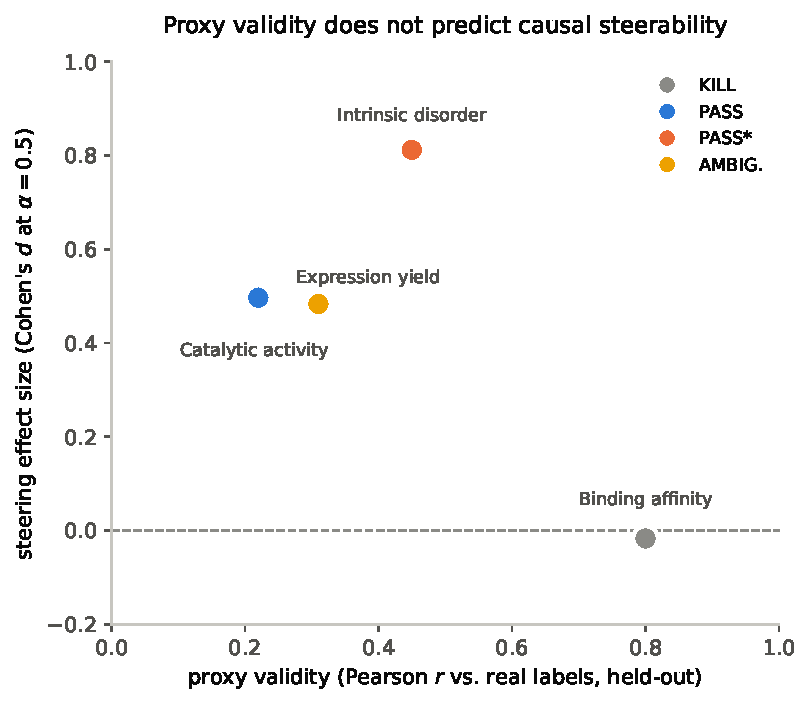
\includegraphics[width=0.68\linewidth]{figures/fig2_proxy_vs_effect.pdf}
\caption{The four runnable targets, plotted as explanatory validity
(proxy Pearson $r$ against real labels) against causal steering effect
size (Cohen's $d$ at $\alpha=0.5$). The most trustworthy explanation
(binding affinity, $r=0.80$) yields the least causally useful
intervention; a far weaker explanation ($r=0.22$, catalytic activity)
yields one of the two most causally effective interventions.}
\label{fig:proxy-vs-effect}
\end{figure}

\textbf{Binding affinity.} Using a ProteinGym deep-mutational-scanning
assay of KRAS binding to a DARPin binder, we build a proxy from
per-position mutational-sensitivity weights learned on the training
split. This is the most rigorously validated explanation in our study:
$r=0.80$ held-out, confirmed by a weight-shuffle null control ($r=-0.001$,
ruling out that the signal is generic rather than position-specific),
held-out-position generalization ($r=0.54$ on positions never seen
during weight-fitting), and mutational-load extrapolation from single to
double mutants ($r=0.70$). The causal intervention built from this
explanation is a flat, unambiguous null at every tested strength, with
zero degenerate sequences -- ruling out generation collapse as an
alternative account. A plausible mechanistic reason
(\S\ref{sec:cases}): this dataset's vector-building groups are
single-backbone point mutants, giving the difference-of-means
construction very little raw compositional signal to act on, independent
of whether the underlying explanation is valid.

\textbf{Catalytic activity.} A glycine-minus-arginine compositional
proxy on DLKcat (cross-protein enzyme turnover data), the weakest
explanation of the four runnable targets ($r=0.22$), matching the
published activity-stability tradeoff in enzymology. This produces a
clean, monotonic causal effect (Figure~\ref{fig:dose-response}, left),
significant at every safe-range $\alpha$, surviving residue-exclusion,
replicated identically across three independent seeds -- the one target
in our sweep with fully unanimous seed-robustness despite the weakest
explanatory grounding.

\subsection{Intrinsic disorder: seed-sensitivity in a robustness criterion}
\label{sec:disorder-detail}

A proxy from the published TOP-IDP disorder-propensity scale
\citep{campen2008topidp} validates at $r=0.45$ (the strongest explanation
in our sweep), confirmed at the per-residue level (AUC $0.71$ via a
sliding window against real per-residue labels) -- a case where
explanatory validity and evaluation rigor are both high. The causal
effect is significant and monotonically dose-responsive on all three
independent seeds (Figure~\ref{fig:dose-response}, right). However, the
residue-exclusion robustness check -- the step analogous to a faithfulness
check on an explanation method -- passes on 2 of 3 seeds (36--42\% of
effect magnitude retained, CI excludes zero) and fails on the third (10\%
retained, CI crosses zero, Figure~\ref{fig:seed-robustness}). The causal
effect's existence and direction are seed-stable; the specific robustness
criterion is not, uniformly.

\begin{figure}[t]
\centering
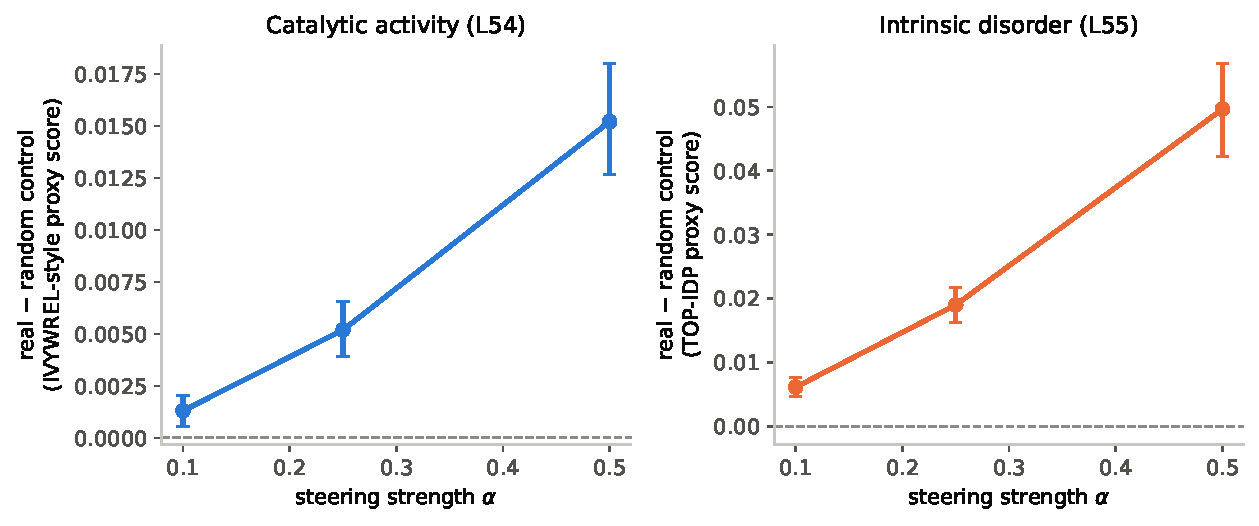
\includegraphics[width=\linewidth]{figures/fig1_dose_response.pdf}
\caption{Dose-response for the two targets passing criterion 2. Both
show a clean, monotonic increase with 95\% bootstrap CIs bounded away
from zero at every point.}
\label{fig:dose-response}
\end{figure}

\begin{figure}[t]
\centering
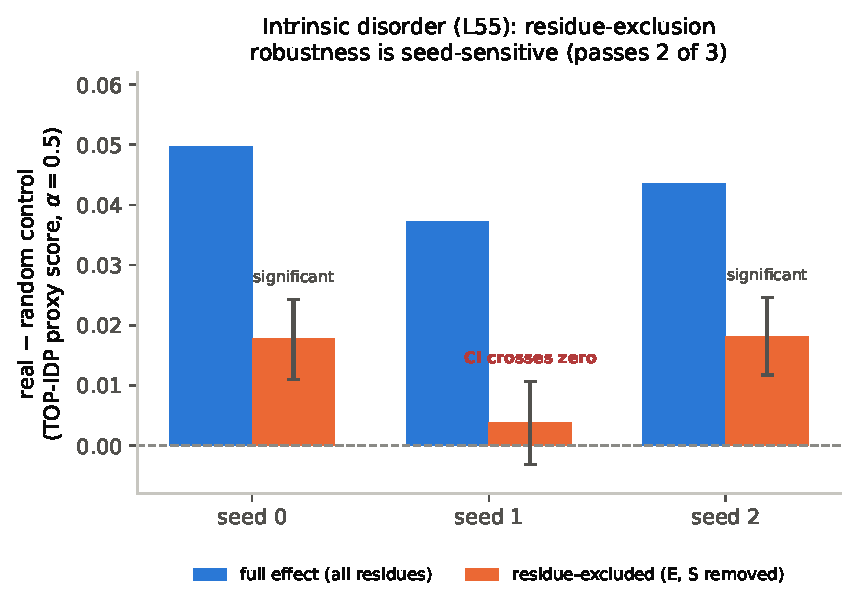
\includegraphics[width=0.7\linewidth]{figures/fig3_seed_robustness.pdf}
\caption{The intrinsic-disorder target's causal effect (blue) and the
same effect after the two dominant substituted residues are excluded
(orange, 95\% bootstrap CIs), across three independent seeds. The
underlying causal effect is stable across all three; the
residue-exclusion faithfulness check is significant on seeds 0 and 2 but
its CI crosses zero on seed 1 -- the same causal effect, the same
robustness criterion, three different verdicts.}
\label{fig:seed-robustness}
\end{figure}

\textbf{Immunogenicity.} We evaluate candidate explanatory proxies
across four tiers of increasing fidelity to the real target. Proxies
predictive on a surrogate binding-affinity tier ($r=0.37$--$0.43$)
collapse to near-chance on the real T-cell-response endpoint
($r\leq0.10$); a full-length-antigen proxy reaching $r=0.38$ is a
source-organism confound -- organism identity alone explains 58\% of the
apparent signal, and the same proxy's correlation flips to $-0.32$ once
organism identity is held out of cross-validation, a direct example of an
explanation that looks physically grounded but is actually tracking an
unrelated confound. No proxy survives criterion 4, so no causal steering
run was performed.

\textbf{Expression yield.} A net-charge-deviation proxy validates at
$r=0.31$--$0.34$ and produces a significant, dose-responsive causal effect
that collapses under residue-exclusion -- an explanation-validity check
that passes but a faithfulness check that fails.

\section{Grounding an Ambiguous Result: A Vector-Geometry Diagnostic}
\label{sec:cases}

Rather than discarding the expression-yield result as unexplained noise,
we compute cosine similarity between its steering vector and every other
target's, layer by layer. We find substantial overlap with the
intrinsic-disorder target's vector: $+0.30$ on the full 33-layer
concatenation, rising to $+0.40$--$0.50$ at the three deepest layers. This
is consistent with the independently documented biology -- disordered
protein regions are known to reduce solubility and expression yield --
and grounds the result causally: expression yield's apparent effect is
best understood as a partial, noisier echo of disorder's already-validated
direction, filtered through a proxy more prone to compositional collapse,
not independent evidence of a sixth causally steerable property. This
diagnostic (compare a new intervention's direction against every other
validated direction in the same study) is a cheap, generalizable
faithfulness check for any study running multiple related causal
interventions.

\textbf{A caught faithfulness-evaluation artifact.} As a mechanistic
follow-up on thermostability, we tested whether restricting steering to
the 5 layers previously identified as causally necessary preserves the
effect of steering all 33. A first evaluation selected its
best-performing $\alpha$ from the full tested range, including
$\alpha\geq1.0$, and concluded the 5-layer subset matched or exceeded the
full intervention. This was an artifact of the evaluation, not a real
result: at that $\alpha$, the 33-layer intervention had already fully
collapsed into degenerate output (zero non-degenerate evaluation
sequences), while the 5-layer subset had not yet collapsed -- an
evaluation methodology issue directly analogous to comparing two
explanation methods at operating points where one has already failed.
Restricting the comparison to a range where neither arm has collapsed and
rerunning end to end gives the honest result: the 5-layer subset produces
a real, residue-robust effect, retaining only 43--59\% of the full effect
size.

The binding-affinity mechanistic account (\S\ref{sec:sweep}) is likewise
grounded, not asserted: the mean per-residue compositional distance
between this target's low/high vector-building groups is $0.003$, versus
$0.02$--$0.05$ for the three cross-protein targets in our sweep -- a
directly measurable reason the causal construction had little signal to
act on, independent of the explanation's own validity.

\section{Related Work}

\citet{huang2025steering} introduce difference-of-means activation
steering for protein language models and validate it causally on
thermostability; we extend their intervention to five new properties
under a pre-registered protocol and test, to our knowledge for the first
time, whether explanatory (proxy) validity predicts causal success across
multiple unrelated properties. \citet{vig2021bertology} identify the
attention head we redo as a genuine causal ablation test, extended here
to a full 480-head sweep with zero correlational information in the
ranking. \citet{adams2025mechanistic} train sparse autoencoders on
ESM-2's residual stream and show, via linear probing -- a purely
correlational, post-hoc attribution method -- that known determinants of
thermostability and subcellular localization are identifiable in SAE
feature space; their one steering experiment is a coherence check (does
steering change fewer residues than a random direction), not a validation
against a real causal ground truth, and their discussion states plainly
that ``investigating how to steer the model in useful ways remains an
open direction for future work.'' Our work answers a version of that
question directly: whether an interpretability method's correlational
validity, evaluated rigorously by the field's own standards, predicts the
causal usefulness of an intervention built on it.

\section{Discussion}

\textbf{What ``causal'' means here.} Every result in this paper is
causal about the model's activation space -- a real intervention on the
forward pass, evaluated against a matched-norm random-direction control
and a residue-exclusion faithfulness check, on generated (not merely
scored) sequences -- not validated against a real biological assay. A
PASS means ``causally steers a validated compositional explanation,'' not
``causally engineers the underlying biological property,'' a distinction
that matters for any claim that an interpretability method's causal
usefulness has been established.

\textbf{Limitations.} All experiments use a single foundation model
(ESM2-650M) at a single scale; we did not test whether these findings
hold at other scales, an open question directly relevant to whether
explanatory-validity/causal-effect mismatches are a property of this
specific model or foundation models more broadly. All proxies are
compositional heuristics rather than learned attribution methods, chosen
for interpretability and speed; a stronger, more sophisticated
explanation method might show a different relationship to causal effect.
We checked seed-robustness for two of five targets; we did not run any
structural or functional plausibility check on generated sequences, so a
PASS does not rule out that causally-steered sequences, while scoring
well on the proxy, are otherwise physically or biologically implausible.

\section{Conclusion}

Correlational validity -- of an attention head's alignment with a known
biological signal, or of a scoring proxy's correlation with real
experimental labels -- does not predict causal effect when a downstream
intervention built on it is actually tested, at two different levels of
the same foundation model class. For interpretability methods intended to
guide scientific discovery or trustworthy intervention in biology, this
argues for validating explanations against the causal interventions they
are meant to support, not treating correlational or attribution-based
salience as self-certifying evidence of causal usefulness.

\bibliographystyle{plainnat}
\bibliography{reference}

\end{document}
